\section{Subsistema de Identificación (ID)}\label{subsisid}
%	\item \textbf{ID: } 
%	El dispositivo RFID es asignado a cada novillo de engorde, y éste lo portará . /*ESTO LO PONGO EN EL QUE YO ESCOGÍ*/
	En el subsistema de Identificación se realiza la identificación de cada novillo mediante un accesorio, característica, marca, descripción, nombre o finalidad. Sin embargo, por cuestiones de recursos, facilidad de uso, utilidad descriptiva e informativa y capacidad de reutilización, se requiere seleccionar una modalidad de las mencionadas en la sección \ref{identiganado}, que cumpla parcial o totalmente con estos criterios.\\
	
	Para seleccionar la alternativa más apropiada se procede a realizar una matriz de selección de peso ponderado bajo los siguientes dictámenes:
	
	\begin{itemize}
	   \item Los pesos asignados para cada criterio son valores enteros del 1 al 5.
	   \item Entre mayor sea el peso asignado, significa que la modalidad es más apropiada para cada criterio de selección.
	   \item \begin{inparaenum}[(i)]
	        Los criterios usados para esta matriz son:
	        \item ``Costo''
	        \item ``Reutilizable''
	        \item ``Manipulable''
	        \item ``Informativo''
	    \end{inparaenum}
	    \item El criterio de costo representa la relación costo beneficio que representa cada alternativa.
	    \item El criterio reutilizable representa la posibilidad de reciclar su uso para futuras ocasiones y que no sea desechable o de único uso.
	    \item El criterio manipulable hace referencia a qué tan intuitivo es y  qué tan fácil es de manejar por terceros.
	    \item En cuanto al criterio Informativo, como su nombre lo indica, éste representa cuán descriptivo e informativo es en cuanto a una res en específico, ya sea por edad, género, raza, todas las anteriores o ninguna.\\
	    
	\end{itemize}
	
	Con base en lo anterior se obtiene la siguiente matriz de pesos:
\begin{table}[H]
\centering
\caption{Matriz de selección por peso ponderado para el subsistema ID. \label{matrizid}}
\begin{tabular}{|c|c|c|c|c|c|}
\hline
\multirow{3}{*}{Alternativas} & \multicolumn{4}{c|}{Criterios} & \multirow{3}{*}{\begin{tabular}[c]{@{}c@{}}Valoración final\\   de la alternativa\end{tabular}} \\ \cline{2-5}
 & 30\% & 25\% & 15\% & 30\% &  \\ \cline{2-5}
 & Costo & Reutilizable & Manipulable & Informativo &  \\ \hline
Arete & 4 & 1 & 4 & 3 & 2,95 \\ \hline
Chip Subcutáneo & 3 & 1 & 4 & 5 & 3,25 \\ \hline
Jáquima / Collar & 5 & 4 & 3 & 1 & 3,25 \\ \hline
Marcado & 4 & 1 & 2 & 2 & 2,35 \\ \hline
Nariguera & 4 & 3 & 2 & 1 & 2,55 \\ \hline
% Jáquima RFID & 5 & 4 & 4 & 5 & 4,6 \\ \hline
\end{tabular}
\end{table}	
% \begin{figure}[H]
% 	\begin{center}
% 		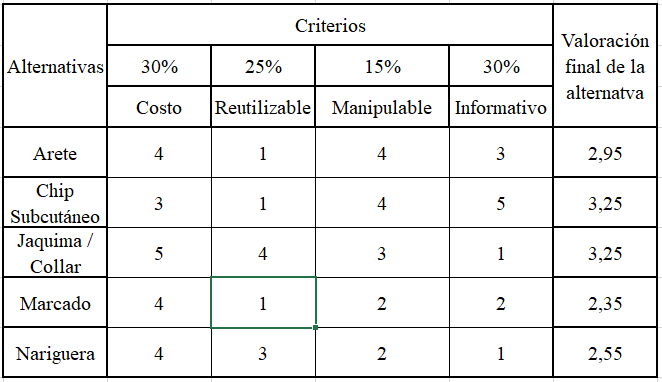
\includegraphics[scale=0.85]{img/matrizid.png}
% 	\end{center}
% 	\caption{Matriz de selección por peso ponderado para el subsistema ID. \label{matrizidpng}}
% \end{figure}


	       % 
	       % 

% De esta forma:}
% \begin{itemize}
%     \item  Respecto al criterio de ``Costo'', un valor de 1 significa que el precio es demasiado elevado ($\frac{\+\$30.000}{Uso}$, aproximadamente) y 5 significa que el precio es económico ($\frac{\-\$10.000}{Uso}$, aproximadamente) para los beneficios que ofrece la alternativa.
%     \item  Respecto al criterio ``Reutilizable'', un valor de 1 significa que la alternativa es desechable mientras que un valor cercano a 5 demuestra que la alternativa puede reutilizarse a futuro ($\frac{\5 Usos}{Unidad}$).
%     \item Respecto al criterio ``Manipulable'', Un valor de 1 significa que la alternativa es difícil de utilizar por terceros mientras que un valor cercano a 5 significa que es intuitiva y amigable para los usuarios (productores o personal ganadero).
%     \item Respecto al criterio ``Informativo'',Un valor cercano a 1 quiere decir que la alternativa puede entregar información subjetiva o ambigua, mientras que un valor cercano a 5 significa que se puede obtener atributos y descripciones pertinentes a una res de ganado de manera eficiente.
% \end{itemize}
	

	
	
	
De esta tabla se puede observar que de las 5 modalidades actuales más utilizadas en la ganadería (ver sección \ref{identiganado}), prevalece el uso de la jáquima o collar y el uso de un chip subcutáneo RFID.
Desde un punto de vista de la ingeniería electrónica, la modalidad que optimiza la identificación del ganado en cuestión de tiempo y facilidad de descripción informativa es la identificación mediante el transponedor de radiofrecuencia. Por otro lado, desde un punto de vista financiero, el uso del chip subcutáneo significa un elevado costo en comparación al uso de Collares que además de ser económicos  pueden ser reutilizables.

No obstante, aunque ambas opciones han resultado ser convenientes, se opta por buscar alternativas que permitan aprovechar los mejores atributos de ambas modalidades. Como resultado se opta por combinar estos atributos en una alternativa híbrida (Jáquima RFID) cuyo análisis y diseño se describe a continuación:

\subsection{Análisis}
 Para esta alternativa híbrida se requiere de 2 partes principales: el punto de lectura RFID, y el accesorio ``RFID tag''. Antes de proponer un primer diseño se opta por observar las condiciones de infraestructura convencional en este tipo de ganado estabulado para disponer de los puntos de lectura y por lo tanto la ubicación física del tag.
  
  \begin{figure}[H]
		\begin{center}
			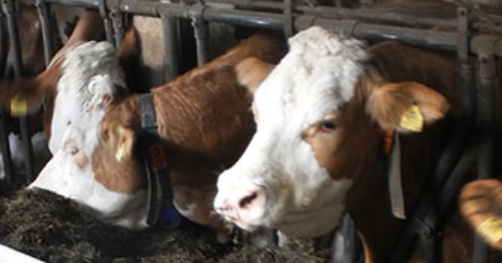
\includegraphics[scale=0.75]{img/barras.png}
		\end{center}
		\caption{Separación de ganado en el comedero.  Tomada de \cite{googlepics}. \label{barraspng}}
	\end{figure}
  
 Como se puede observar en la Figura \ref{barraspng}, el ganado estabulado se encuentra separado entre sí mediante puestos individuales de alimentación a los que son ingresados. Además, accede a su alimento al pasar su cabeza y cuello a través de un arreglo de barras que bordean la nuca; este arreglo varía de forma y tamaño acorde al tipo de res y se utiliza para evitar disputas en la manada.\\
 \begin{inparaenum}[(i)]
	        Con base en lo anterior se puede establecer que el lector RFID deberá estar posicionado en:
	        \item  Dentro o fuera del puesto de alimentación individual.
	        \item  En algún punto del arreglo de varillas que bordea la nuca del animal.
 \end{inparaenum}
 
 
\subsection{Diseños}
% \begin{itemize}
	\subsubsection{Diseño 1, Arnés, Chaleco ó ``Backband''}
	En primera instancia se considera un chaleco usable, portable y reutilizable, que sería utilizado por cada individuo perteneciente al ganado estabulado desde su ingreso hasta su salida en la etapa de ceba; es decir, hasta que alcance un peso adecuado para ser transformado en carne para consumo humano y una vez esto ocurriera, el chaleco sería reasignado a un próximo nuevo miembro de la etapa de engorde.
		
	Como los equinos, bovinos y otros animales domésticos ya utilizan accesorios en su día a día, se consideró posible que el ganado usase este tipo de complemento. Por otra parte, uno de los objetivos principales de este proyecto es que se pueda identificar cada una de las reses de manera automática y eficiente, por lo que el uso de etiquetas RFID (ver Figura \ref{rfidtagpng}) fue uno de los influyentes más importantes en este diseño.
	
	\begin{figure}[H]
	\begin{center}
		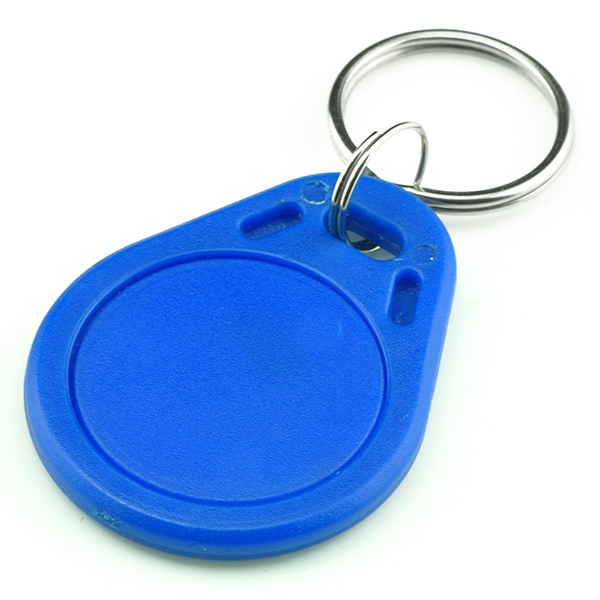
\includegraphics[scale=0.25]{img/rfidtag.png}
	\end{center}
	\caption{Etiqueta ó ``Tag'' RFID. Tomada de \cite{googlepics}. \label{rfidtagpng}}
	\end{figure}

% Ahora bien, en la infraestructura general de un comedero para ganado estabulado, se tienen algunas observaciones que por lo general son añadidas a la misma, como por ejemplo, la separación de cada cabeza mediante barras a los costados que sirven para separar a los animales entre sí evitando disputas en la manada (Ver Figura \ref{barraspng}).
%   Estas barras también rodean la nuca del animal dejando un espacio apropiado para que éste pueda ingresar su cabeza y cuello hasta el comedero.
% de canoa, canaleta o mixto.

% 		\begin{figure}[H]
% 		\begin{center}
% 			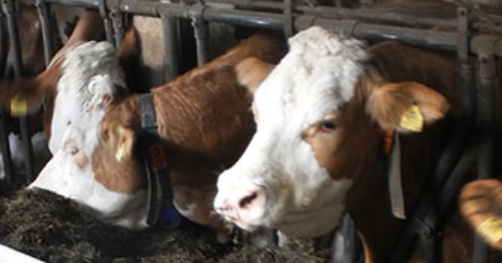
\includegraphics[scale=0.55]{img/barras.png}
% 		\end{center}
% 		\caption{Separación de ganado en el comedero. \label{barraspng}}
% 		\end{figure}
		
Además, para no requerir de un encargado de la lectura de cada ``RFID tag'' en los chalecos, es necesario que el lector se encuentre en una posición fija. Con esto en mente, se presupuso que el lector debería estar en un punto estratégico que facilitara la proximidad de la etiqueta RFID sin incomodar al individuo que sería alimentado.\\

Por lo tanto, el lector RFID se encontraría en la barra superior que bordea la nuca del bovino y por consiguiente la etiqueta RFID del chaleco se encontraría cerca de la ultima vértebra cervical.

Se diseñó un primer bosquejo en 3D del chaleco que contendría la etiqueta RFID y de la cual se colocarían las correas ajustables que bordearían el cuerpo del novillo (Ver Figura \ref{mod1png}),  

		\begin{figure}[H]
		\begin{center}
			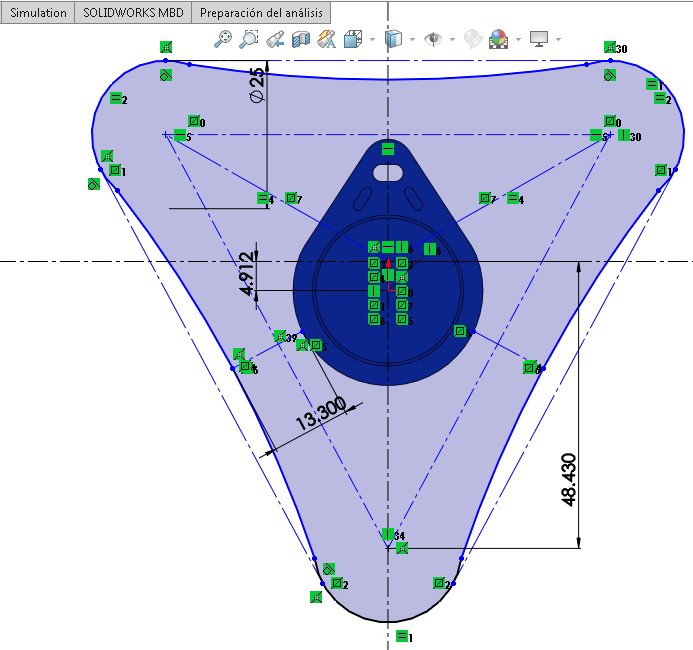
\includegraphics[scale=0.45]{img/primermodel.png}
		\end{center}
		\caption{Primer modelo 3D del compartimento RFID. \label{mod1png}}
		\end{figure}

Lastimosamente se detectó una primer falencia a este diseño, esto debido a que no todas las razas de bovinos más usados en este tipo de ganadería en Colombia son iguales en altura, contextura y fisionomía \cite{razas}. En la Figura \ref{jorobapng} se puede observar razas como la Cyr, Brahman y Nelore; estas poseen una especie de joroba en la nuca o tejido descolgado en la parte inferior del cuerpo, lo que complica el uso de los chalecos y de la posición de la etiqueta RFID en ellos.

		\begin{figure}[H]
		\begin{center}
			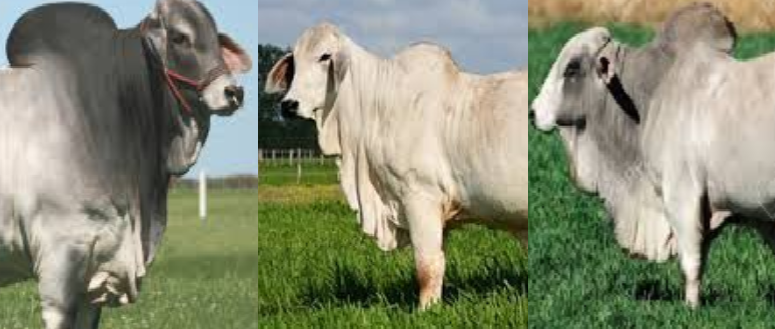
\includegraphics[scale=0.7]{img/joroba.png}
		\end{center}
		\caption{Fisionomía de razas comunes en el ciclo productivo de la Carne. Tomada de \cite{fisio1}. \label{jorobapng}}
		\end{figure}

\subsubsection{Diseño 2, ``Armband''}
Como medida reactiva o correctiva al problema del diseño anterior, se consideró que la etiqueta RFID podría ubicarse a uno de los costados de las extremidades del individuo y por ende el lector tendría una nueva ubicación acorde a este cambio. No obstante se presentaron otras complicaciones que evidenciaron fallas en este diseño.

La abrazadera ubicada en la extremidad, dificulta el movimiento articular de la misma y como en cualquier otro caso de interacción animal que vive en grupo, se presentan ocasiones de confrontación física entre sujetos del sexo masculino; estas confrontaciones pueden suponer un daño irreparable en el compartimento portable del ``Armband'' dificultando la identificación del bovino en ocasiones futuras.\\
		
% 	\end{itemize}
		
\textit{\textbf{Anotación:} Para conservar factores característicos como la portabilidad, usabilidad, reutilización del identificador RFID y recalcando lo aprendido sobre las falencias de los diseños anteriores, se decide combinar el uso de la Jáquima y los 2 prototipos diseñados con la etiqueta RFID dando como resultado el siguiente diseño:}

\subsubsection{Diseño 3, ``Jáquima RFID''}
 
Para el diseño de este nuevo prototipo se observa que un rasgo físico común entre las razas de bovinos usadas para engorde, es  que poseen un gran espacio en la parte frontal del cráneo, por encima de los ojos y que suelen usarse jáquimas comerciales, convencionales, modificables, etc.\\

En la figura \ref{argollapng} se observa que las Jáquimas especializadas utilizan una argolla de conexión para unir y tensionar las correas ajustables. Teniendo esto presente, se puede reemplazar o adaptar un accesorio que se acople a las correas y que pueda portar una etiqueta RFID.

		\begin{figure}[H]
		\begin{center}
			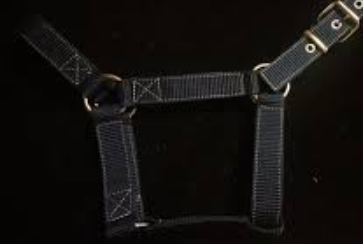
\includegraphics[scale=0.9]{img/argolla.png}
		\end{center}
		\caption{Argolla de conexión. \label{argollapng}}
		\end{figure}

Nuevamente, el diseño 3D de este accesorio se realiza en SolidWorks. En este caso, el diseño requiere de 2 partes. Primeramente se diseña la base, a la que se le condiciona un corte interno que sirve como almohadilla en donde se inserta la etiqueta RFID y también cuenta con 3 hendiduras para el acople de la tapa protectora.

        \begin{figure}[H]
		\begin{center}
			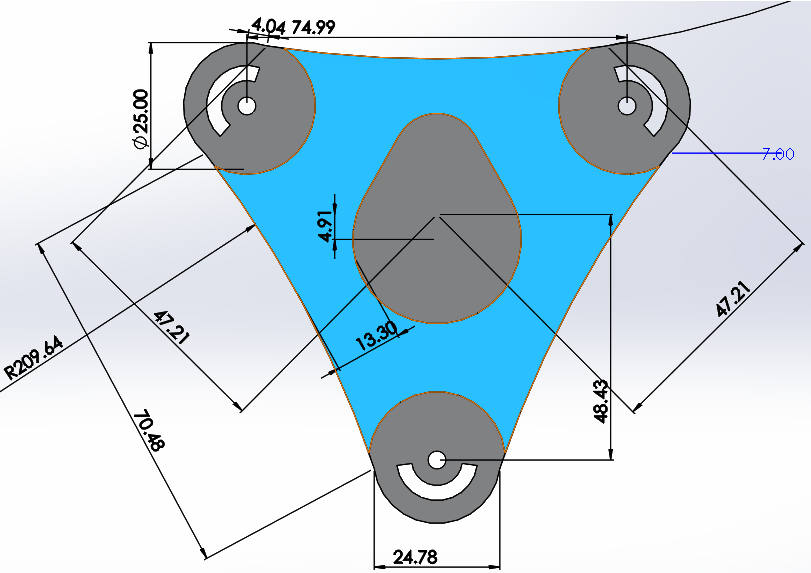
\includegraphics[scale=0.635]{img/medidasbase.png}
		\end{center}
		\caption{Medidas para la Base. \label{medidasbasepng}}
		\end{figure}

Así mismo la tapa protectora cuenta con 3 salientes que sirven para acoplarse correctamente a la base y permitir que se conforme el accesorio en su totalidad. En  el lado derecho de la Figura \ref{tapabasepng} se observa la primera parte usada como base y del lado izquierdo, la otra parte que servirá de tapa protectora.

        \begin{figure}[H]
		\begin{center}
			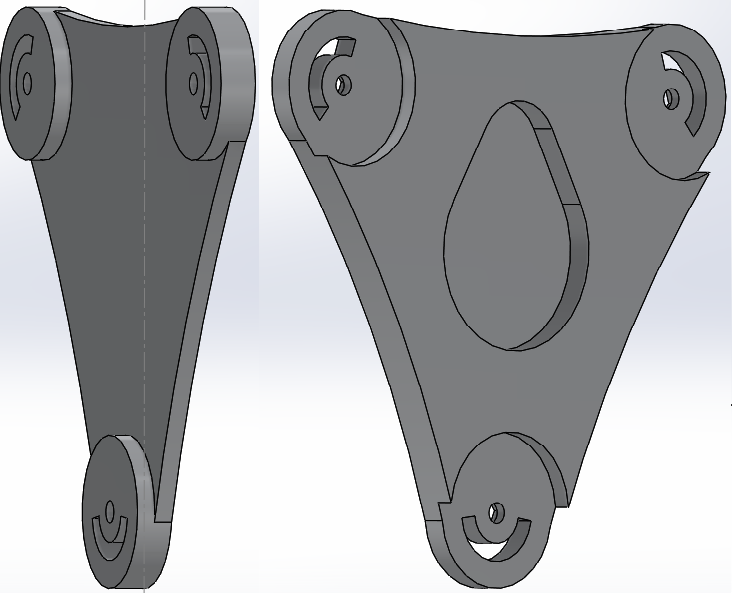
\includegraphics[scale=0.55]{img/tapabase.png}
		\end{center}
		\caption{Tapa y Base del accesorio para la Jáquima RFID. \label{tapabasepng}}
		\end{figure}

Es importante añadir que este accesorio permite cambiar la etiqueta RFID si lo requiere, lo que evidencia la reutilización del prototipo para ganado en el futuro.\\

Finalmente, al ensamblar la base y la tapa del accesorio junto con unas abrazaderas ajustables, se finiquita el accesorio prototipo denominado como ``Jáquima RFID''. Este contiene un identificador único (UID) que se encuentra grabado en la memoria de la etiqueta RFID añadida al mismo.
%   para la identificación del ganado estabulado:

\begin{figure}[H]
	\begin{center}
		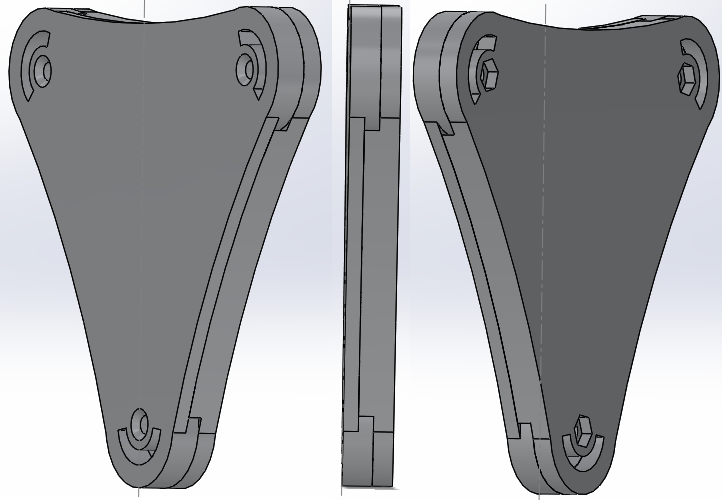
\includegraphics[scale=0.55]{img/jaquimaidsimul.png}
	\end{center}
	\caption{Jáquima ID. \label{jaquimaidpng}}
\end{figure}

% \end{itemize}

 Por su parte para este último diseño se requiere que el lector del dispositivo RFID deba posicionarse en un lugar que esté en contacto con la parte frontal del novillo. Siguiendo este orden de ideas y teniendo en cuenta que se presentarán distintos ejemplares de diferentes tamaños y fisonomías; el punto estratégico de lectura sería la puerta de ingreso al puesto de comida. Además, como los animales son guiados a estos puestos con la ayuda de personal calificado, el registro en la entrada es el punto más apropiado para garantizar que el individuo ingresado está (o no) identificado para su alimentación y estudio correspondiente.
Así pues, se concluyen los diseños de este subsistema satisfaciendo la O.I \#\ref{OI1} y el objetivo especifico #4 donde los novillos que cuenten con este accesorio podrán ser debidamente identificados a la hora de ser ingresados a los puestos de comida donde se les dosifica el alimento.
\pagebreak
% Con base en lo anterior se incluye este diseño como alternativa dentro de la tabla \ref{matrizid} obteniéndose un peso ponderado superior debido a que se logran aprovechar las mejores características posibles.

% \begin{table}[H]
% \centering
% \begin{tabular}{|c|c|c|c|c|c|}
% \hline
% \multirow{3}{*}{Alternativas} & \multicolumn{4}{c|}{Criterios} & \multirow{3}{*}{\begin{tabular}[c]{@{}c@{}}Valoración final\\   de la alternativa\end{tabular}} \\ \cline{2-5}
%  & 30\% & 25\% & 15\% & 30\% &  \\ \cline{2-5}
%  & Costo & Reutilizable & Manipulable & Informativo &  \\ \hline
% Arete & 4 & 1 & 4 & 3 & 2,95 \\ \hline
% Chip Subcutáneo & 3 & 1 & 4 & 5 & 3,25 \\ \hline
% Jáquima / Collar & 5 & 4 & 3 & 1 & 3,25 \\ \hline
% Marcado & 4 & 1 & 2 & 2 & 2,35 \\ \hline
% Nariguera & 4 & 3 & 2 & 1 & 2,55 \\ \hline
% Jáquima RFID & 5 & 4 & 4 & 5 & 4,6 \\ \hline
% \end{tabular}
% \caption{Matriz de selección por peso ponderado para el subsistema ID final. \label{matrizidfinal}}
% \end{table}	
